
\section{Spel \& lekar}

\fancypagestyle{Spel & lekar}{
    \fancyhead{} % clear all header fields
    \fancyhead[LE,RO]{\textbf{Spel \& lekar}}
}
\pagestyle{Spel & lekar}



\subsection*{\textbf{Fuck U}}

%//Från bonkboken känns som en gammel släkting till ring of fire???

Dra kort i tur från en kortlek. Följ regeln från listan under
och möjligtvis egna ettablerade regler (se 2)

Regler:

Ess: Dela ut en klunk (Var sportslig)

2: Regelkort. Hitta på en regel eller ändra/tabort en regel. \textbf{EJ grundreglerna eller något personligt.}

3-6: Dela ut antalet klunkar som det står på kortet.

7: Räknekort. Den som drar kortet börjar med att högt säga "1"
och den vänster fortsätter då med "2".
Så håller man på tills någon antigen säger något som är
delbart med 7 eller innehåller en 7:a. t.ex. 14 eller 17.
Missar man eller tvekar drickar man.

8: Pissekort. Sparas tills man använder det. Man lägger in kortet om man måste på toa.

9: Tumkort. Sparas tills det används.
Den som har kortet sätter när de vill upp sin tumme på bordet
och håller den där och resten följer efter.
Sist dricker

10: "Fuck you"-kort.
Sparas tills det används. Den som har kortet säger han de vill "Fuck U", den som säger det sist dricker.

Kn: Frågekort. Den som drar detta börjar med att ställa fråga till någon
och den personen ska direkt ställa en nu fråga till någon
annan som spelar. Ställer man tillbaka en fråga, tvekar, svarar
eller ställer en fråga so mredan ställts dricker man.

D: Temakort. Man säger ett tema och så går man runt i
ringen och alla får säga något som har med temat att göra.
Kan man inte, tvekar eller om man säger något som redan sagts dricker man.

K:Sparas till alla kungar dragits. Om en person får alla fyra kungar får alla andra svepa vad de har i glaset/flaskan.
Annars får den som drar sista kungen svepa.
\subsection*{\textbf{Caps}}

\textbf{Caps} (\emph{Capsning}) är ett alkoholhaltigt dryckesspel som
går ut på att kasta kapsyler i glas. Spelet kan spelas med minst två
till åtta spelare. Spelet spelas sittande på golvet/marken i en ring,
där varje spelare har med sig ett antal alkoholhaltiga drycker.

Förberedelser

Innan spelet börjar placeras ett glas i mitten av ringen, detta kallas
mittenglaset, vilket fylls upp med dryck motsvarande höjden av två
fingrar från varje spelare eller tills mittenglaset är fyllt, beroende
på vilket som kommer först. Varje spelare fyller därefter upp varsitt
spelglas \textbf{upp till höjden av två fingrars bredd} med valfri
dryck. Dessa spelglas placeras därefter i en ring runt mittenglaset, så
nära som möjligt.

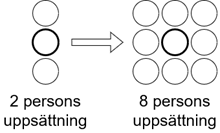
\includegraphics[width=2.29167in,height=1.38819in]{media/CapsPositions.png}

Samtliga spelare sätter sig därefter i en ring, fördelaktigt i
skräddarställning (benen i kors) med en benlängds avstånd ifrån sina
spelglas och med en bra mängd kapsyler till hands.

Spelregler -- Turnerings Caps

\begin{quote}
\emph{OBS! Det finns lokala variationer på caps över hela Sverige, men
dessa regler gäller främst för capsning i Västerås.}
\end{quote}

\begin{enumerate}
\def\labelenumi{\arabic{enumi}.}
\item
  Den deltagare som har flest avklarade studieår börjar capsa. Är det
  lika mellan flera spelare så är det den äldsta spelaren som börjar.
  \underline{Turordningen följer klockan}, alltså åt vänster.
\item
  För att ett caps-kast ska räknas som giltigt måste armbågen nudda knät
  under hela kastet, och vinkeln mellan kastarmens över- och underarm
  får inte överstiga 90 grader innan capsen släpps.
\item
  \textbf{Granncaps.} Om det är 5 eller flera spelare i ringen, gäller
  reglerna för ``\textbf{granncaps}''. Det innebär att du inte får capsa
  på glasen som tillhör spelarna direkt till vänster eller höger om dig
  förrän du har capsat ut alla andra deltagare i ringen. Om man bryter
  mot denna regel räknas det som en ``\textbf{felcaps}''. I så fall
  måste den spelare som capsade fel dricka ur sitt egna spelglas, tömma
  det på kapsyler, fylla det på nytt med dryck och sedan går turen
  vidare till nästa sperlare. (Se regel 1. för turordning)
\item
  Om en spelare A träffar ett giltigt glas på korrekt sätt med sin caps,
  initieras en duell. Spelare B, vars glas har blivit träffat, ska då
  försöka träffa glaset som tillhör spelare A, som initierade duellen.
  Detta fortsätter fram och tillbaka tills någon missar

  \begin{enumerate}
  \def\labelenumii{\alph{enumii}.}
  \item
    Om spelare B (den utmanade) missar motståndarens glas först räknas
    det som en ``\textbf{miss}''. Spelare B måste då dricka ur sitt
    spelglas, tömma det på kapsyler och fyller upp det igen med dryck.
    Därefter tar spelare B ut sitt glas från ringen, och spelare A
    fortsätter capsa på annan spelare.
  \item
    Om spelare A (den som initierade duellen) missar först, måste
    spelaren dricka ur sitt spelglas, tömmer glaset på kapsyler och
    fyller det på nytt med dryck. Efter detta ställer samtliga spelare i
    ringen tillbaka sina spelglas, och capsen går vidare till nästa
    spelare i turordningen. (Se regel 1. för turordning)
  \item
    Om spelare A lyckas capsa ut samtliga spelare i ringen, har spelare
    A ``\textbf{kingat}''. Det innebär att alla spelare i ringen,
    förutom från spelare A, ska säga ''\emph{\textbf{all hail the
    king}}'', dricker sitt spelglas igen och fyller dem på nytt.
    Därefter ställer alla tillbaka sina spelglas i ringen, och capsen
    går vidare till nästa spelare i turordningen.
  \end{enumerate}
\item
  Om en spelare träffar mittenglaset vid en initiering, ska alla spelare
  i ringen dricka upp sina spelglas. Samtidigt ska spelaren som träffade
  mittenglaset också dricka upp mittenglaset och tömma det på kapsyler.
  Under tiden sjunger alla spelare:
\end{enumerate}

\begin{quote}
\emph{\textbf{Vi skålar för våra vänner och dom som vi inte
känner}}

\emph{\textbf{Och dom som vi inte känner, de sätter vi på}}

\emph{\textbf{Hej ho, hej ho, de sätter vi på}}

\emph{\textbf{Hej ho, hej ho, de sätter vi på}}

\textbf{\emph{SKÅL!}}
\end{quote}

\begin{enumerate}
\def\labelenumi{\alph{enumi}.}
\item
  Om mittenglaset däremot träffas under en duell så räknas det som en
  \textbf{miss} (se regel 4.a \& 4.b).
\end{enumerate}

\begin{enumerate}
\def\labelenumi{\arabic{enumi}.}
\setcounter{enumi}{5}
\item
  Om en kapsyl lyckas landa i ett spelglas på ett sådant sätt att den
  flyter på ytan, kan en spelare kalla på ``\textbf{sänkning}''. Då
  måste spelaren, vars spelglas kapsylen flyter i, hälla i dryck tills
  kapsylen inte längre flyter.
\item
  Om mängden kapsyler i spelglaset är så stor att en kapsyl ligger
  ovanför ytan, kan en spelare kalla på ``\textbf{gravsten}''. Då måste
  spelaren, vars spelglas kapsylen ligger i, fylla på med dryck tills
  kapsylen inte längre är ovanför ytan.
\item
  Under \textbf{turneringscaps} gäller ``\emph{\textbf{last man
  standing}}''. Reser man på sig för att t.ex. sträcka på benen, hämta
  mer dryck eller gå på toaletten, är man ute ur spelet och turneringen.
  Detta gäller även om man spyr eller beter sig allmänt otrevligt. Om du
  däremot har problem med att få kontakt med en spelare av olika
  anledningar, kan man kasta en kapsyl \textbf{lätt} på denna person.
  Detta räknas \textbf{inte} som allmänt otrevligt beteende, då
  ändamålet enbart är att få kontakt med personen.
\item
  Under \textbf{turneringscaps}, om två ringar tillsammans har totalt 7
  spelare, slås ringarna ihop. Då får deltagarna i den \textbf{minsta}
  ringen resa sig upp och direkt gå och sätta sig i den andra ringen.
\end{enumerate}

\begin{quote}
\textbf{NOTERA} att inga toalettpauser är tillåtna under ringbytet.
\end{quote}

Variant -- Socialcaps/vänskapscaps

Reglerna för socialcaps är mycket liknande reglerna för turneringscaps,
med några få tillägg och ändringar.

\begin{enumerate}
\def\labelenumi{\arabic{enumi}.}
\item
  Under socialcaps kan varje spelare istället fylla sitt spelglaset med
  vatten och ha ett separat dryckesglas bredvid sig, där man kan fyller
  valfri dryck och dricka från.
\item
  Under socialcaps är det mer acceptabelt att ställa sig upp för att
  t.ex. gå på toaletten eller hämta mer dryck. En spelare som ställer
  sig upp åker inte ur spelet, utan kan återkomma och sätta sig i ringen
  igen.
\end{enumerate}


\subsection*{\textbf{Threeman}}

Threeman är ett spel med ett bräde, tärningar och en hattdjävel. När man blir
tilldelad klunkar av någon som kan spelet ska man dricka dessa.

Regler:

\begin{enumerate}
    \item Man får endast berätta den första regeln
    \item[...]
\end{enumerate}

\subsubsection*{Varianter:}

\subsubsection*{Reglerverk (Lila/Gula/Randiga)}

När spelet börjar deklareras regelverket och reglerna följer därefter

\subsubsection*{Phösar-Threeman}

Lägg till tärning(ar)

Deklarera vem som har högst HP

\subsubsection*{Phantom-Threeman}

Ta bort tärning(ar)

\subsubsection*{Threeman med Raoke}

En Raoke deklareras och bär en hatt

\newpage

\subsection*{\textbf{Fuck the Dealer}}

Tillbehör:

Folk, dryck, kortlek

En dealer kollar på det översta kortet i en kortlek och frågar personen till vänster vilken valör kortet har. Gissar dom rätt dricker dealern 10 klunkar. Gissar dom fel säger dealern om kortet är högre eller lägre än gissningen. personen gissar då igen. Gissar dom rätt dricker dealern 5 klunkar. Gissar dom fel så dricker spelaren mellan skillnaden av deras gissning och kortet. Kortet läggs sedan på bordet för alla att se.

Lyckas dealern inte bli tilldelar klunkar av tre personen i rad flyttas kortleken vidare medsols och en den nya dealern börjar där den gammla slutade.

Variant:

Kung eller ess

Eftersom hur mycket man själv dricker är beroende på Deltat av kortet som drogs och sin gissning spelar LTD ofta under förståelsen att det bara kan finnas kungar och ess i leken. Även om detta inte visar sig vara sant när kortet vänder på sig.

\subsection*{\textbf{Knucklebones}}

Materiell:

18 tärningar eller 1 tärning och papper, penna \& Suddigummi\\

Två spelare har motstående 3x3 bräden. Gå i tufr och rullar en tärning. Placera tärningen (Värdet på tärningen) i en av rutorna.

Lägger du en tärning som matchar en tärning i din motståndares kollumn så kan du ta bort deras tärningar av samma värde i den kolumnen.

När någon spelare fyller hela sitt bräde avslutas matchen.

Dina poäng är summan av alla dina tärningar. Tärningar av samma värde i samma kolumn multipliceras med antalet tärningar av det värdet. t.ex. en kolumn med 2st 3or och en 2a är värd (3+3)*2+(2)*1 = 14

\subsubsection*{Variant: 4 Spelare}

För att öka spelplanen till att tillåta 4 spelare så säts den upp med 4st 3x3 bräden så varje spelare har en motståndares bräde diagonalt från sin egna.

Spelet fortsätter som vanligt med additionen att om en tärning du lägger matchar en av dina motståndares tärningar över diagonalen så tas de bort. 

När någon av spelarna lyckas fylla sitt bräde är spelet över och poäng beräknas som vanligt.

\newpage